\chapter{Evaluation}\label{chap:results}
In this chapter, we will conduct a comprehensive evaluation of our proposed BiBEx system. Given that BiBEx is an ensemble of multiple machine learning models, processing steps, and pipelines, each performing their specific tasks, we decided to evaluate the entire system using both intrinsic and extrinsic approaches.\\
In the intrinsic evaluation (Section~\ref{sec:results_intrinsic}), we will assess the individual components within our system. This includes evaluating the performance of our Document Segmentation Model, Reference Parser Model, and Author Parser Model.\\
In the extrinsic evaluation (Section~\ref{sec:results_extrinsic}), we will assess how the overall BiBEx system functions as a unified entity. We will evaluate the system's capability to extract document authors and references.\\
By conducting both intrinsic and extrinsic evaluations, we aim to gain a comprehensive insight of the performance and capabilities of our proposed BiBEx system, demonstrating its effectiveness in extracting metadata from scholarly publications.

\section{Intrinsic Evaluation}\label{sec:results_intrinsic}
In this section, we explore the evaluation process of our system components, namely the Document Segmentation Model, Reference Parser Model, and Author Parser Model. To assess the performance of these models, we compared their outputs against reference models.\\
For each component model, we established one or multiple reference models that are well-established and widely accepted within the field. By comparing the outputs of our models with these reference models, we can quantify the performance of our system components.


\subsection{Document Segmentation Model}\label{sec:eval_docseg}
To optimize our Document Segmentation Model, we tuned our hyperparameters using a 5-fold cross-validation combined with grid search. The hyperparameters that yielded the best performance were determined as follows: learning rate = 1e-4, batch size = 4, and warm-up ratio = 0.1.\\
With the optimized hyperparameters, we trained the Document Segmentation Model on the entire training set. Subsequently, we compared the model's results against various reference models to evaluate its performance. Among these reference models were mBERT~\cite{hug_cased_bert} and XLM-Roberta~\cite{hug_xlmr}, which are well-established transformer models, utilized in various NLP tasks, as explored in Chapter~\ref{chap:background}. Additionally, we also tested a CRF model, which are employed in applications such as GROBID for document segmentation.\\
Table~\ref{tab:results_document_segment_compare} shows these results. Figures~\ref{fig:results_final_docseg_cls} and \ref{fig:results_final_docseg_conf} show the results and the confusion matrix of the final model utilized by BiBEx. Table~\ref{tab:results_docseg_lang} gives an overview of the model's performance on the DocBank and GEOcite portion of the test set.

\begin{table}[!ht]
\centering
\begin{tabular}{|l|
>{\columncolor[HTML]{DAE8FC}}l |
>{\columncolor[HTML]{EFEFEF}}l |
>{\columncolor[HTML]{DAE8FC}}l |
>{\columncolor[HTML]{EFEFEF}}l |}
\hline
\textbf{label}     & \textbf{LayoutXLM} & \textbf{mBERT} & \textbf{XLM-RoBERTa} & \textbf{CRF} \\ \hline\hline
abstract           & \textbf{0.932}     & 0.894          & 0.878                & 0.784        \\ \hline
author             & \textbf{0.922}     & 0.828          & 0.86                 & 0.768        \\ \hline
caption            & \textbf{0.92}      & 0.640          & 0.659                & 0.662        \\ \hline
equation           & \textbf{0.760}     & 0.607          & 0.702                & 0.623        \\ \hline
figure             & 0.746              & 0.725          & \textbf{0.762}       & 0.698        \\ \hline
footer             & \textbf{0.847}     & 0.804          & 0.783                & 0.733        \\ \hline
paragraph          & \textbf{0.973}     & 0.952          & 0.952                & 0.937        \\ \hline
reference          & \textbf{0.986}     & 0.96           & 0.98                 & 0.911        \\ \hline
section            & \textbf{0.888}     & 0.67           & 0.697                & 0.581        \\ \hline
table              & \textbf{0.854}     & 0.691          & 0.721                & 0.615        \\ \hline
title              & \textbf{0.929}     & 0.864          & 0.864                & 0.765        \\ \hline\hline
F1 macro           & \textbf{0.92}      & 0.814          & 0.805                & 0.734        \\ \hline
F1 micro           & \textbf{0.968}     & 0.936          & 0.936                & 0.864        \\ \hline
\end{tabular}
\caption{A comparison of our fine-tuned LayoutXLM model and various reference models. Depicted are F1-scores.}
\label{tab:results_document_segment_compare}
\end{table}

\begin{table}[!ht]
\centering
\begin{tabular}{|l|
>{\columncolor[HTML]{DAE8FC}}l |
>{\columncolor[HTML]{EFEFEF}}l |
>{\columncolor[HTML]{DAE8FC}}l |}
\hline
\textbf{label}              & \textbf{Total} & \textbf{DocBank} & \textbf{GEOcite} \\ \hline\hline
abstract                    & 0.932          & \textbf{0.985}   & 0.866            \\ \hline
author                      & 0.922          & \textbf{0.924}   & 0.902            \\ \hline
caption                     & 0.92           & \textbf{0.965}   & 0.797            \\ \hline
equation                    & 0.760          & \textbf{0.76}    & 0.0              \\ \hline
figure                      & 0.746          & \textbf{0.992}   & 0.717            \\ \hline
footer                      & 0.847          & 0.832            & \textbf{0.849}   \\ \hline
paragraph                   & 0.973          & \textbf{0.98}    & 0.964            \\ \hline
reference                   & 0.986          & 0.983            & \textbf{0.991}   \\ \hline
section                     & 0.888          & \textbf{0.904}   & 0.872            \\ \hline
table                       & 0.854          & \textbf{0.917}   & 0.834            \\ \hline
title                       & 0.929          & \textbf{0.984}   & 0.899            \\ \hline\hline
F1 macro                    & 0.92           & \textbf{0.93}    & 0.79             \\ \hline
F1 micro                    & 0.968          & \textbf{0.973}   & 0.95             \\ \hline
\end{tabular}
\caption{The resulting F1-scores of the fine-tuned LayoutXLM model reported on the DocBank and GEOcite portion of our test set.}
\label{tab:results_docseg_lang}
\end{table}

\begin{figure}[bp!]
    \centering
    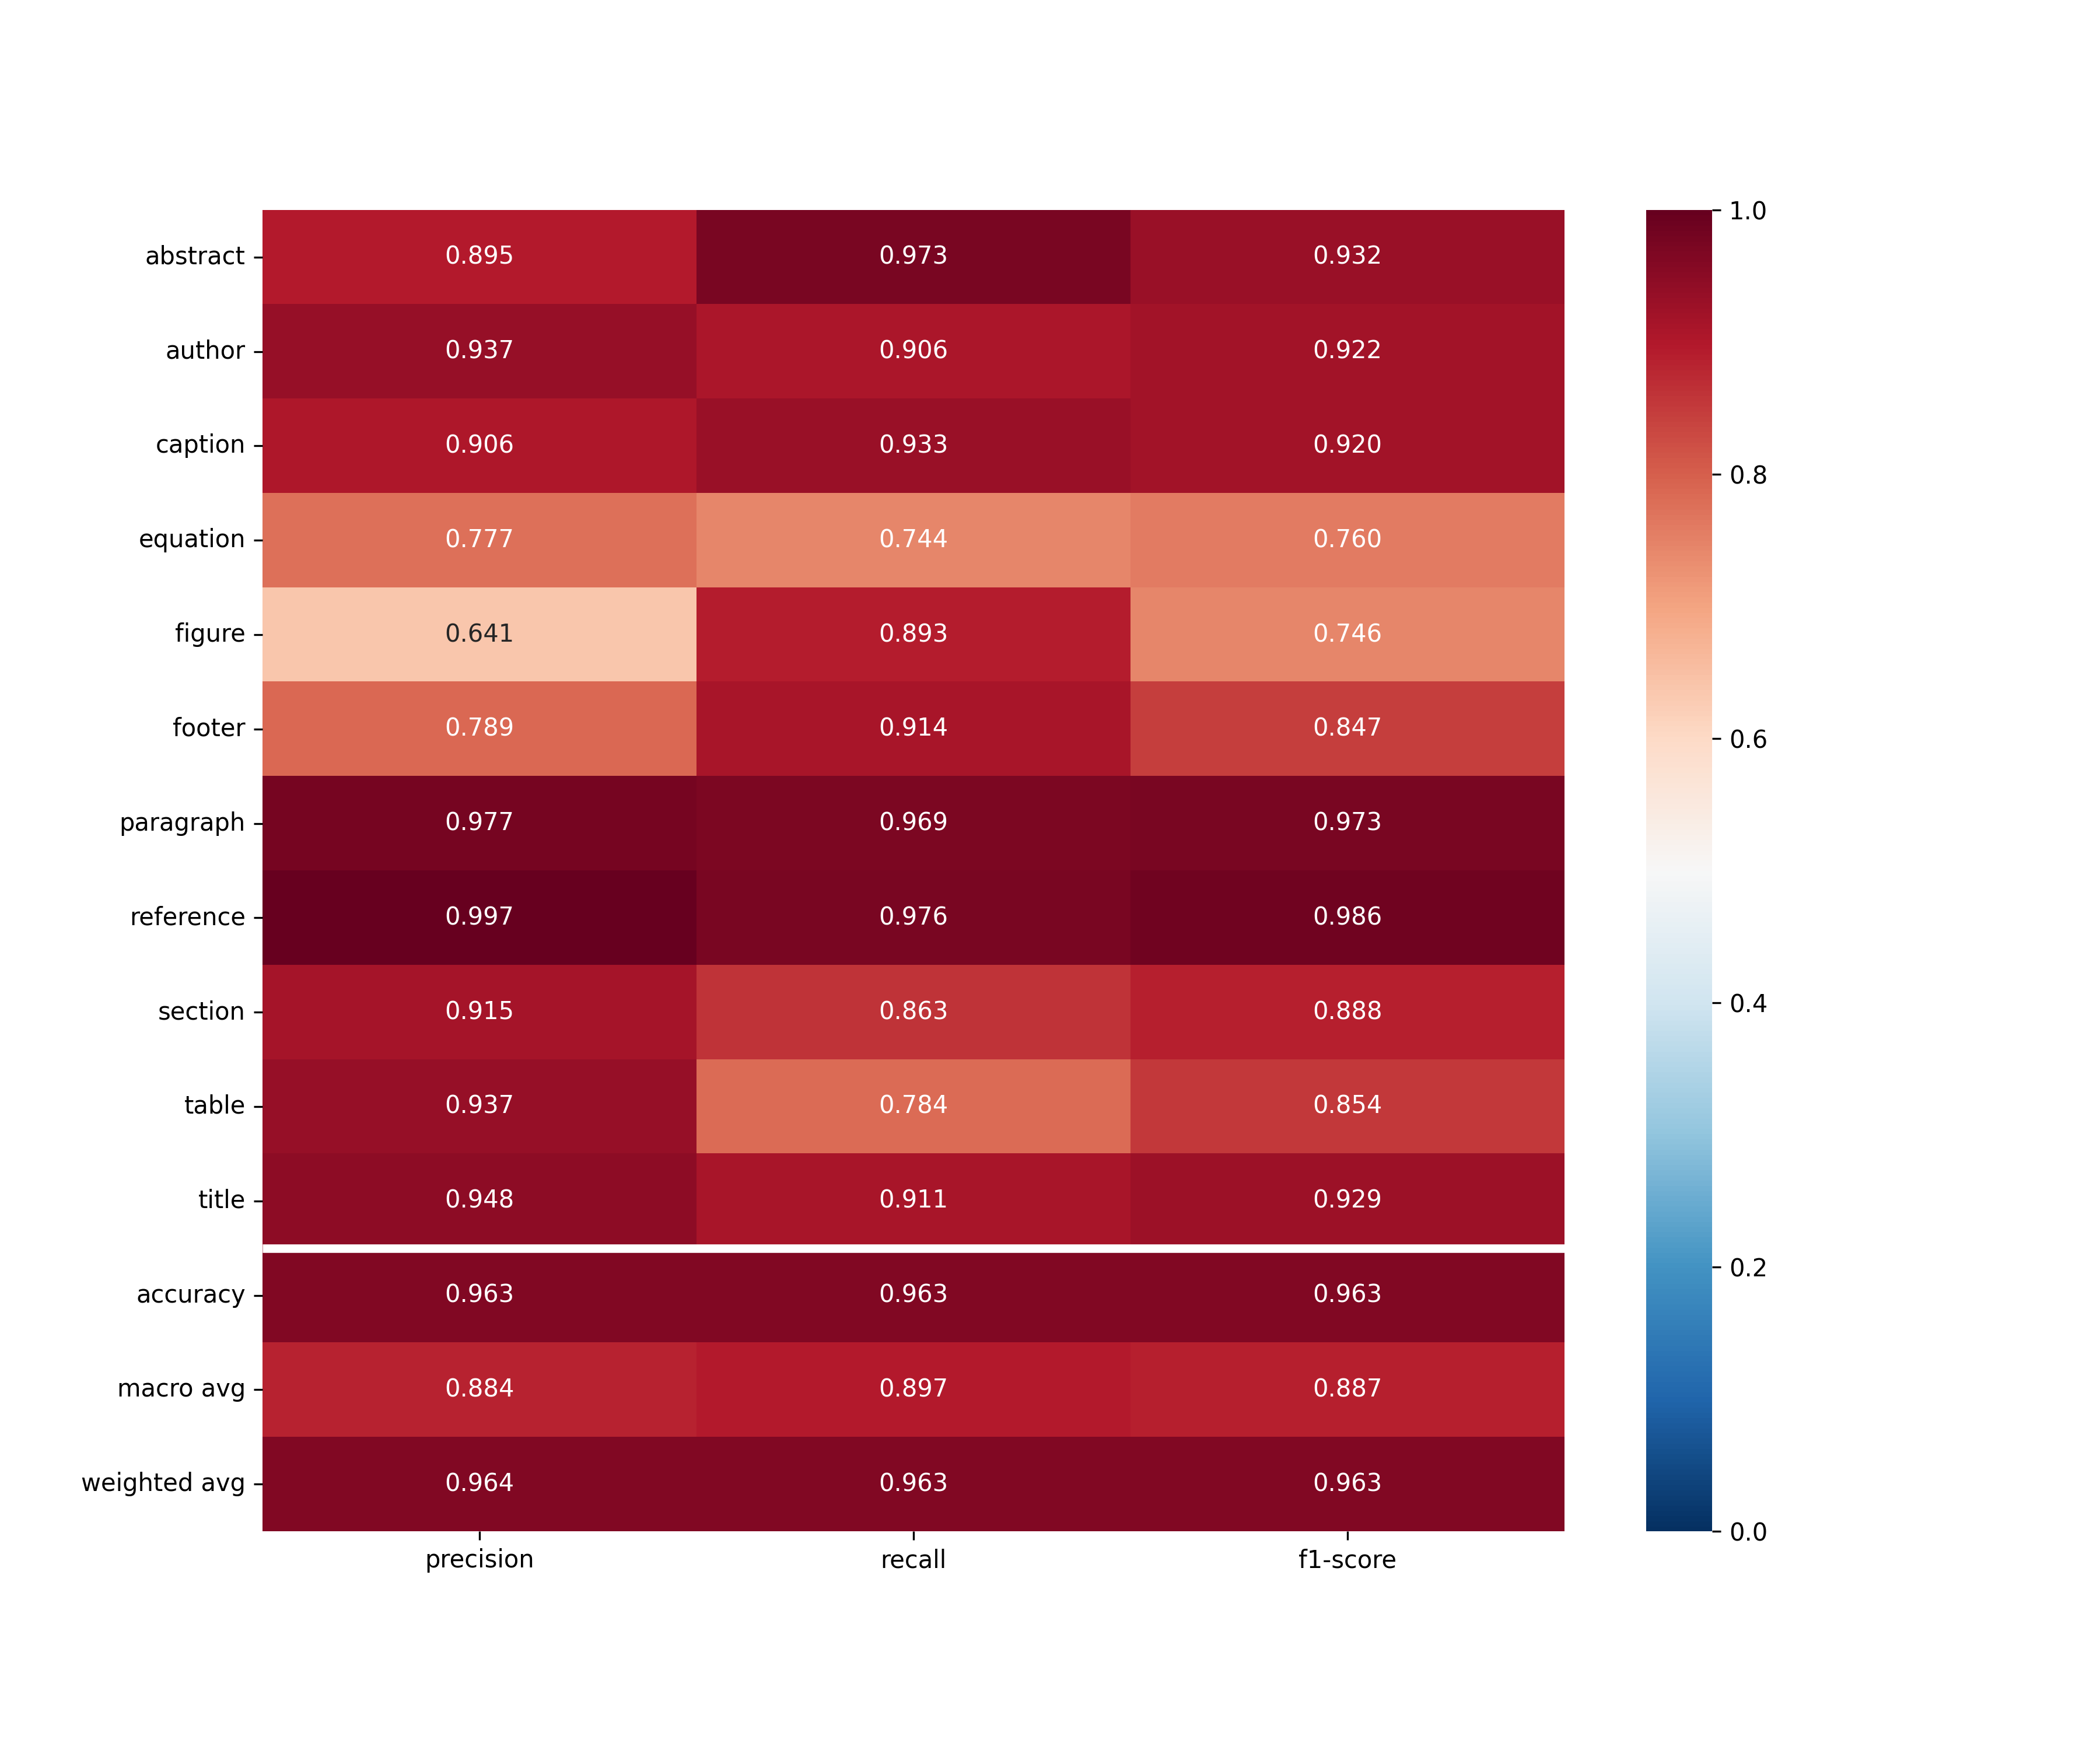
\includegraphics[trim=2cm 0 4cm 0, width=1.0\linewidth]{images/results/document_segmentation/docseg_cls_report_all.png}
    \caption{The resulting precision, recall, and F1-scores of our Document Segmentation Model utilized in BiBEx.}
    \label{fig:results_final_docseg_cls}
\end{figure}

\begin{figure}[bp!]
    \centering
    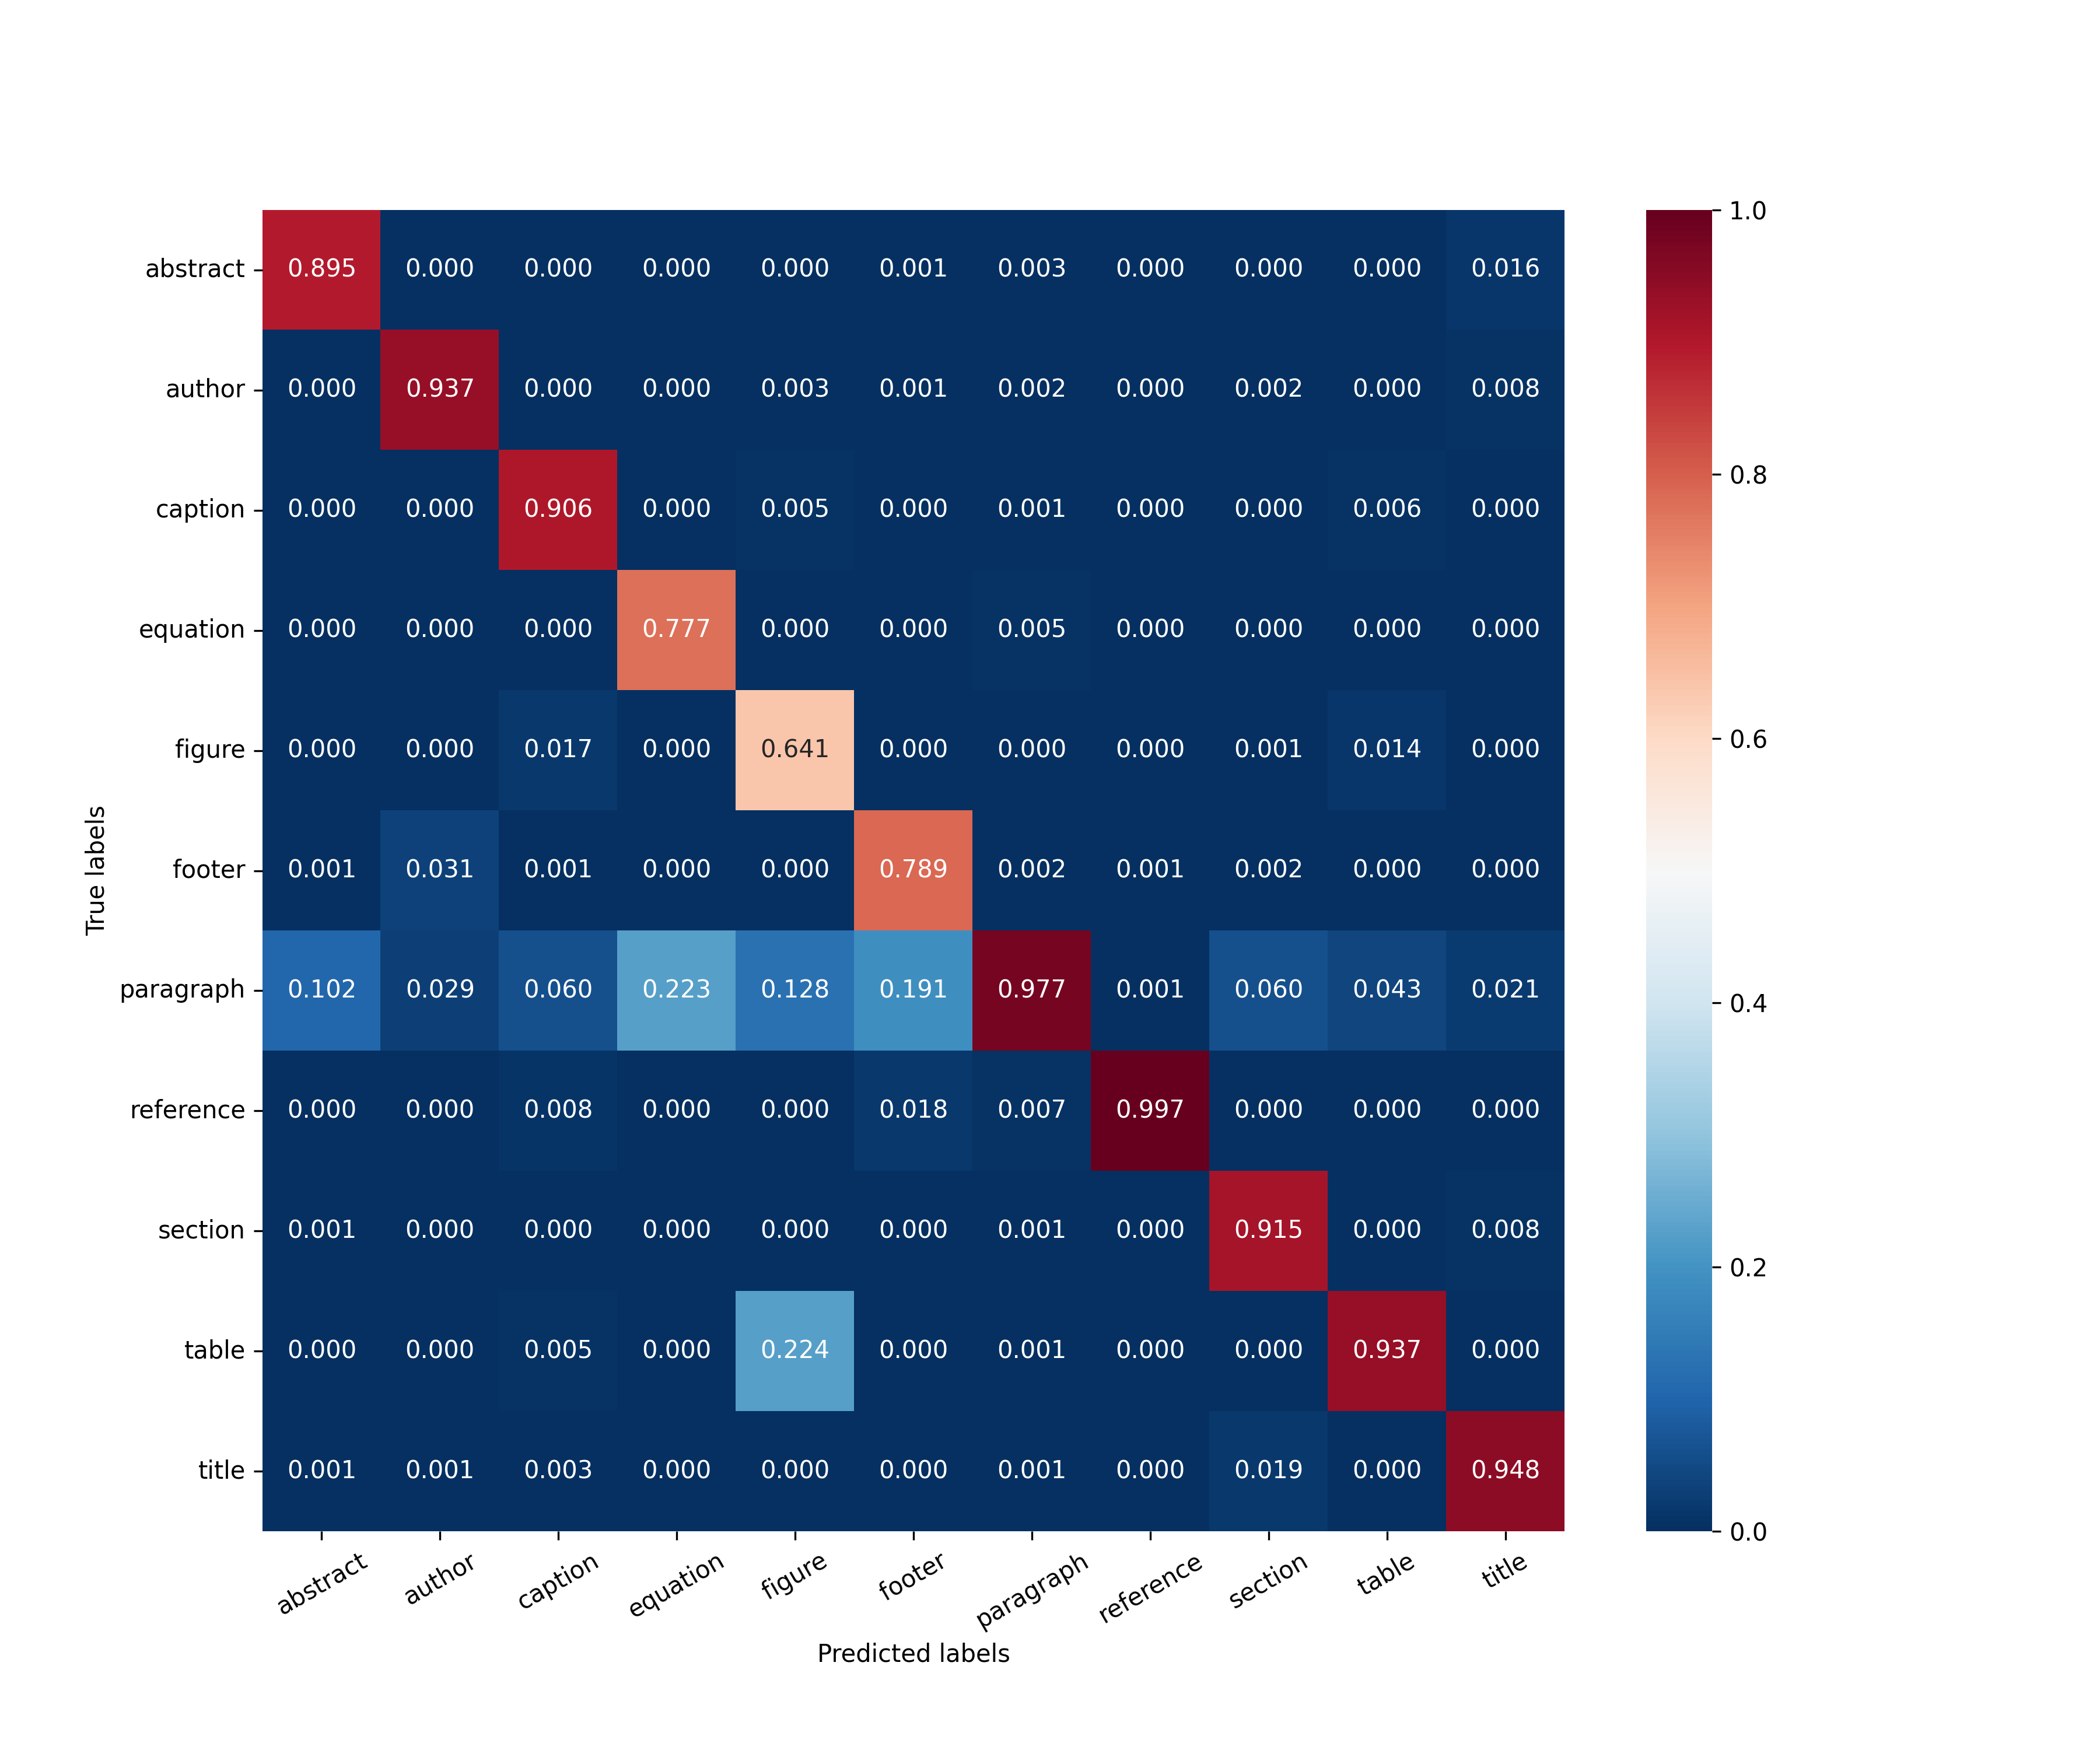
\includegraphics[trim=2cm 0 4cm 0, width=1.0\linewidth]{images/results/document_segmentation/docseg_conf_matrix_norm_pred_all.png}
    \caption{A confusion matrix, normalized over the predicted labels, of the Document Segmentation Model utilized in BiBEx.}
    \label{fig:results_final_docseg_conf}
\end{figure}
\FloatBarrier

\subsection{Reference Parser Model}\label{sec:eval_refseg}

Similar to our Document Segmentation Model in Section~\ref{sec:eval_docseg}, we optimized our hyperparameters using a grid search 5-fold crossvalidation. The hyperparameters that performed best were determined as follows: learning rate = 1e-5, batch size = 8, and epochs = 2. The $\alpha$ value to weight the loss function between the two outputs was set to $1.0$.\\
After optimizing the hyperparameters, we trained the Reference Parser Model using the entire training data and evaluated its performance by comparing its results against a mBERT~\cite{hug_cased_bert} and CRF model. The features utilized in the CRF model, were similar to those reported by Boukhers et al.~\cite{excite_methods} during the training of the EXparser system.\\
After analyzing the performance of our reference models, we implemented our custom classification head for the XLM-RoBERTa model. The results of both of the model's outputs, the label prediction and the new reference prediction, are depicted in Figures~\ref{fig:results_final_refseg_cls} and \ref{fig:results_final_refseg_ref}. A comparison of the entity prediction results of all models is visualized in Table~\ref{tab:results_refseg_compare}.

\begin{table}[!ht]
\centering
\begin{tabular}{l|
>{\columncolor[HTML]{DAE8FC}}l |
>{\columncolor[HTML]{EFEFEF}}l |
>{\columncolor[HTML]{DAE8FC}}l |}
\hline
\multicolumn{1}{|l|}{\textbf{label}}    & \textbf{CRF} & \textbf{mBERT} & \textbf{XLM-RoBERTa} \\ \hline\hline
\multicolumn{1}{|l|}{author}    & 0.743        & 0.877          & \textbf{0.891}       \\ \hline
\multicolumn{1}{|l|}{editor}    & 0.449        & 0.882          & \textbf{0.895}       \\ \hline
\multicolumn{1}{|l|}{fpage}     & 0.967        & 0.960          & \textbf{0.984}       \\ \hline
\multicolumn{1}{|l|}{issue}     & 0.706        & 0.715          & \textbf{0.847}       \\ \hline
\multicolumn{1}{|l|}{lpage}     & 0.980        & 0.974          & \textbf{0.983}       \\ \hline
\multicolumn{1}{|l|}{other}     & 0.695        & 0.758          & \textbf{0.795}       \\ \hline
\multicolumn{1}{|l|}{publisher} & 0.690        & 0.831          & \textbf{0.845}       \\ \hline
\multicolumn{1}{|l|}{source}    & 0.767        & 0.842          & \textbf{0.860}       \\ \hline
\multicolumn{1}{|l|}{title}     & 0.775        & \textbf{0.869} & 0.868                \\ \hline
\multicolumn{1}{|l|}{url}       & 0.753        & 0.500          & \textbf{0.907}       \\ \hline
\multicolumn{1}{|l|}{volume}    & 0.904        & 0.870          & \textbf{0.939}       \\ \hline
\multicolumn{1}{|l|}{year}      & 0.968        & 0.973          & \textbf{0.980}       \\ \hline\hline
\multicolumn{1}{|l|}{micro avg} & 0.816        & 0.876          & \textbf{0.907}       \\ \hline
\multicolumn{1}{|l|}{macro avg} & 0.783        & 0.838          & \textbf{0.899}       \\ \hline
\end{tabular}
\caption{A comparison of the entity prediction of our fine-tuned XLM-RoBERTa model and two reference models. Depicted are F1-scores.}
\label{tab:results_refseg_compare}
\end{table}

\begin{figure}[bp!]
    \centering
    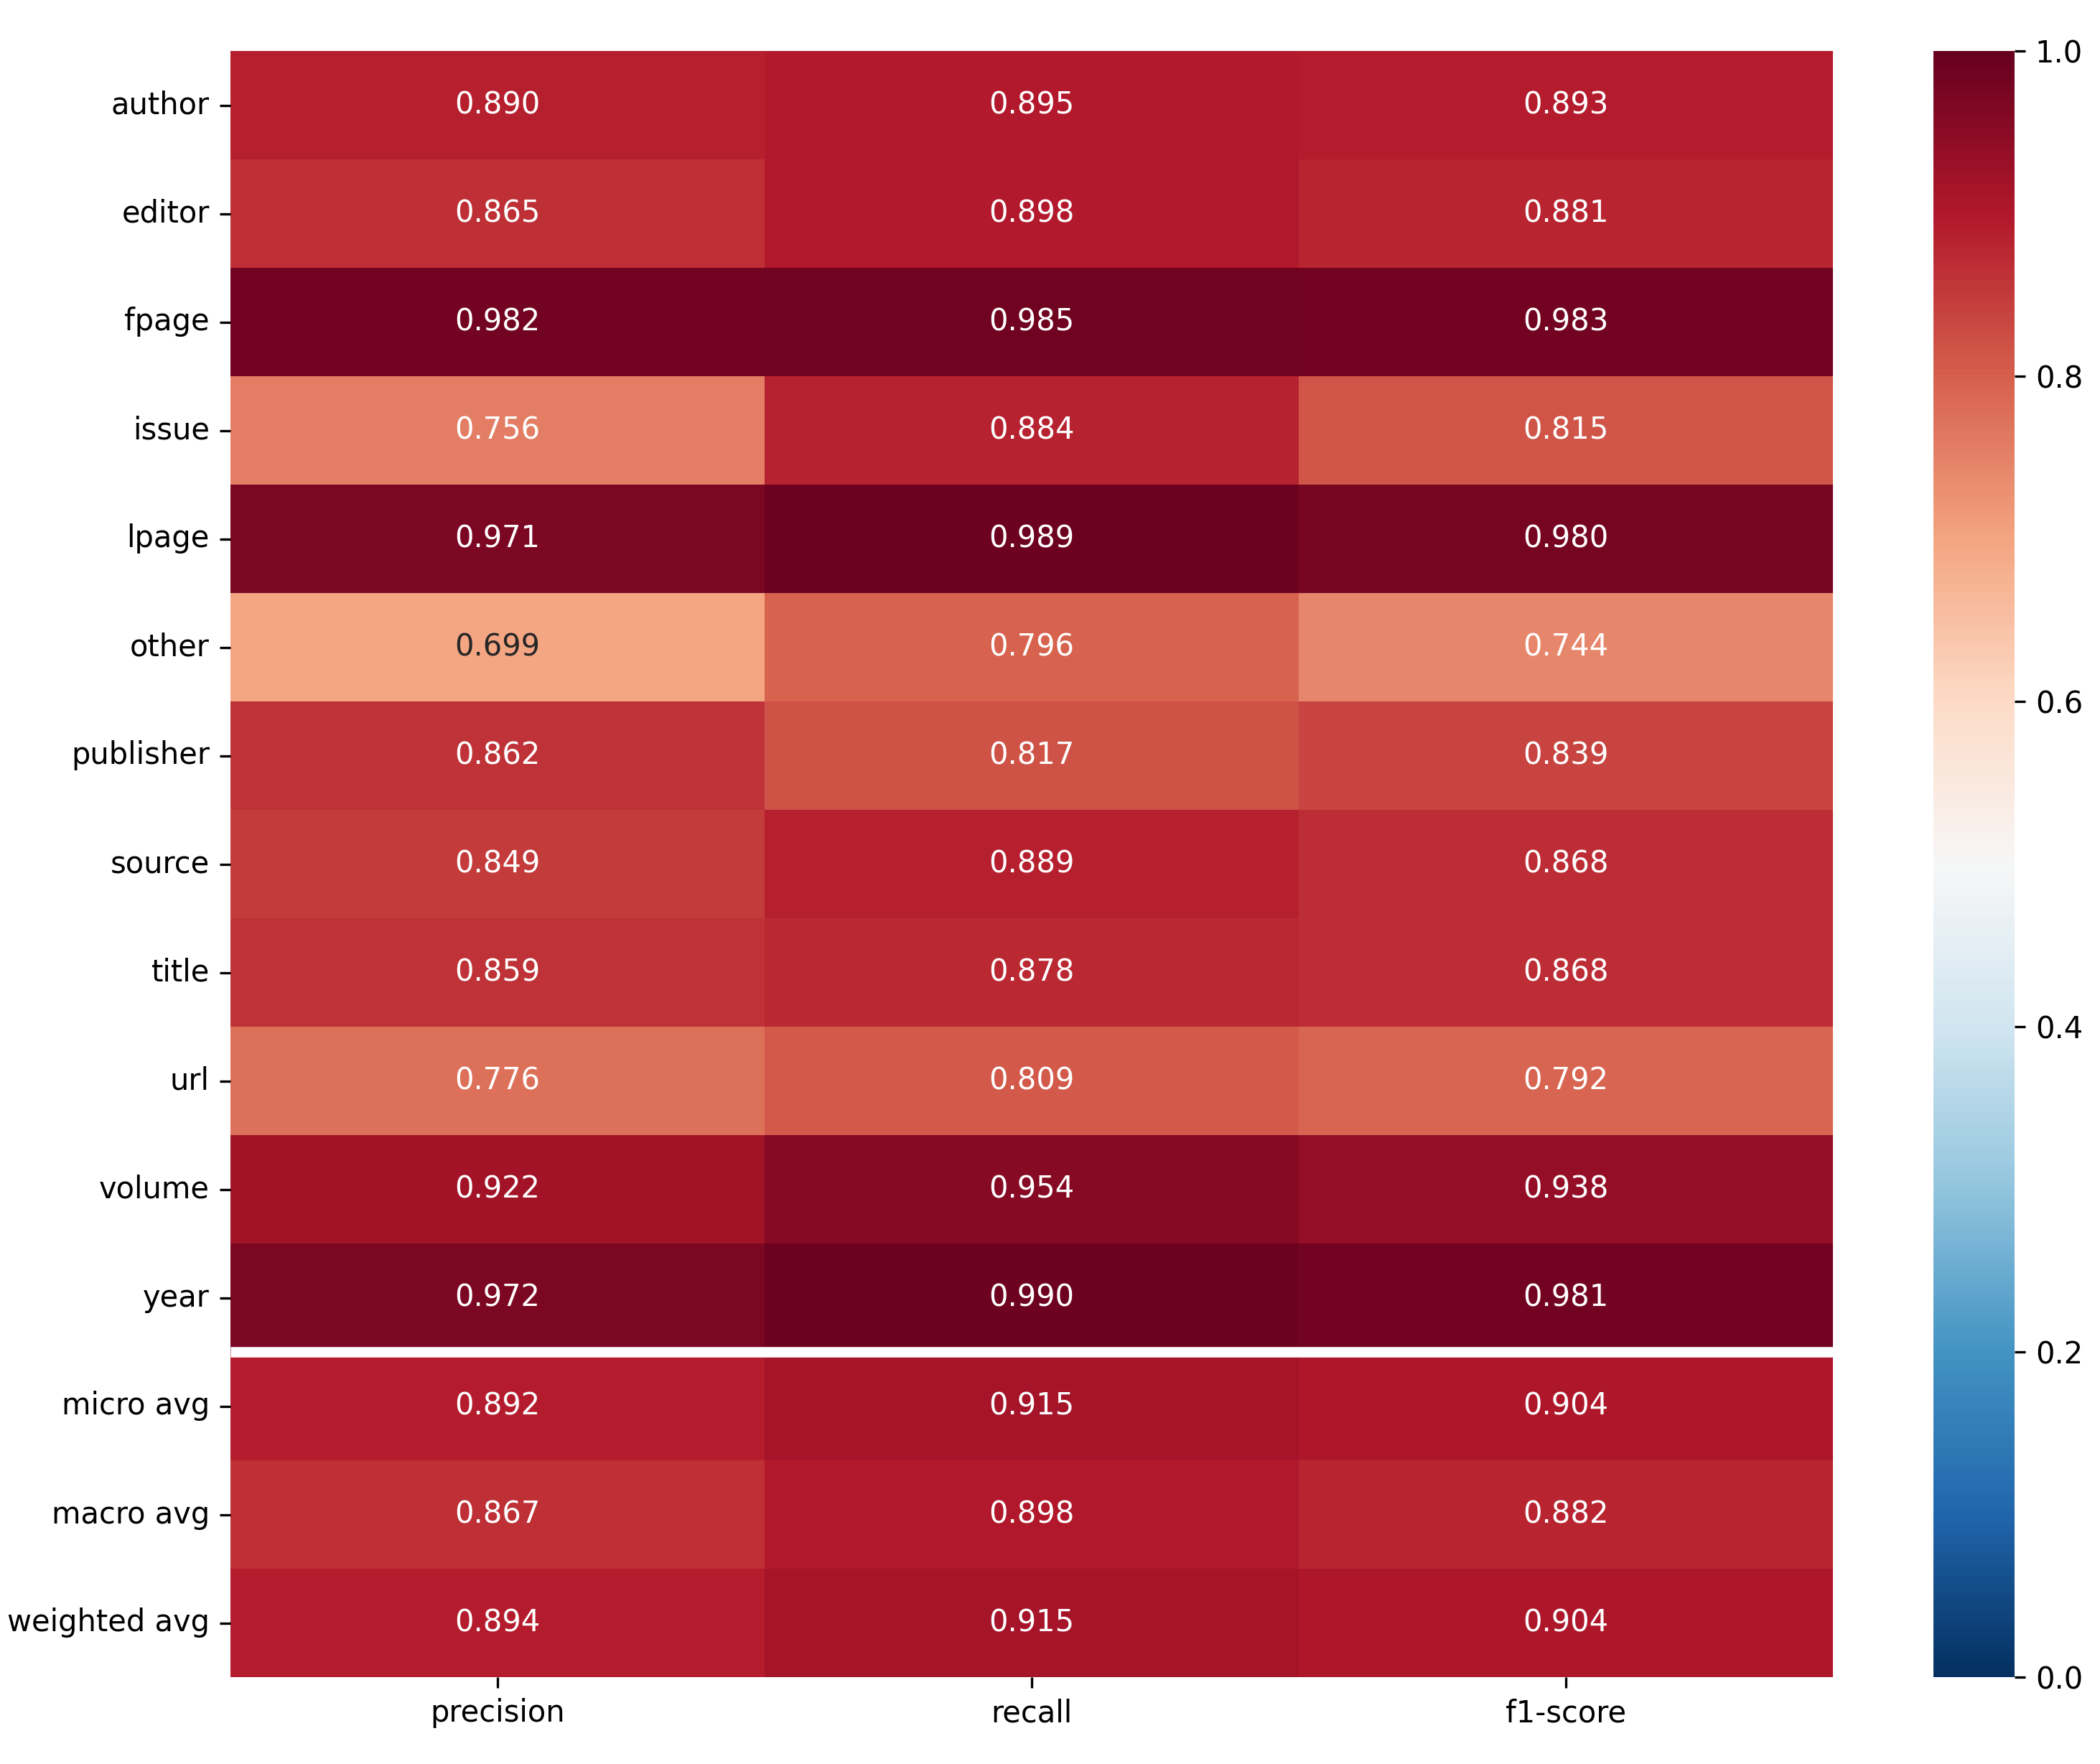
\includegraphics[width=1.0\linewidth]{images/results/reference_parser/ref_seg_cls_croped.png}
    \caption{The resulting precision, recall, and F1-scores of our Reference Parser Model utilized in BiBEx. Reported are the results of the entity prediction connected layer.}
    \label{fig:results_final_refseg_cls}
\end{figure}

\begin{figure}[bp!]
    \centering
    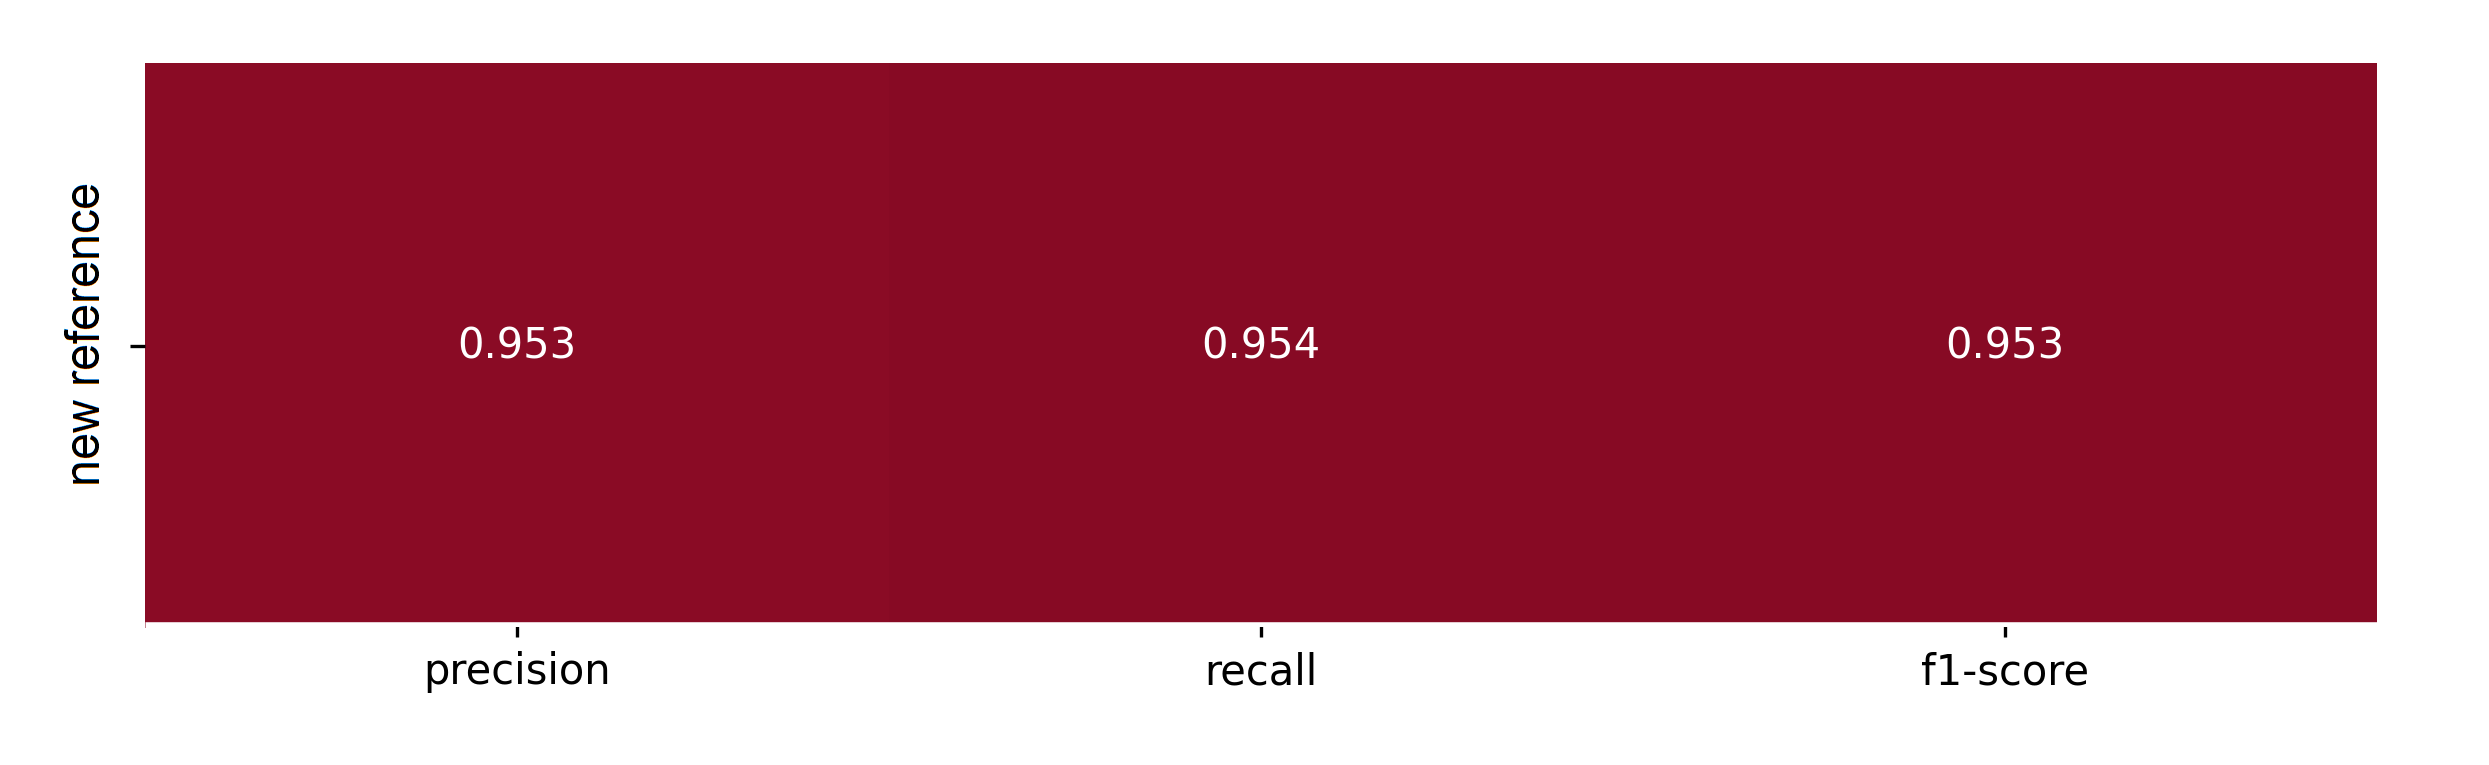
\includegraphics[width=0.8\linewidth]{images/results/reference_parser/ref_seg_croped.png}
    \caption{The resulting precision, recall, and F1-score of the connected layer, predicting a new reference of our Reference Parser Model utilized in BiBEx.}
    \label{fig:results_final_refseg_ref}
\end{figure}

\FloatBarrier

\subsection{Author Parser Model}
Equivalent to our our previous models in Section~\ref{sec:eval_docseg} and \ref{sec:eval_refseg}, we searched for the best hyperparameters utilizing a grid search with 5-fold crossvalidation. The selected hyperparameters are: learning rate = 5e-5, batch size = 16, and epochs = 2.\\
After optimizing our hyperparameters, we trained the Author Parser Model using our whole training set and evaluated its performance by comparing its results against a XLM-RoBERTa~\cite{hug_xlmr} and CRF model, as visualized in Table~\ref{tab:results_author_comp}. We further depict the performance of our final Author Parser Model in Figure~\ref{fig:results_author_cls} and visualize its results on various languages in Table~\ref{tab:results_author_lang}.

\begin{table}[!ht]
\centering
\begin{tabular}{l|
>{\columncolor[HTML]{DAE8FC}}l |
>{\columncolor[HTML]{EFEFEF}}l |
>{\columncolor[HTML]{DAE8FC}}l |}
%l|l|l|}
\hline
\multicolumn{1}{|l|}{\textbf{label}}                          & \textbf{CRF} & \textbf{mBERT} & \textbf{XLM-RoBERTa} \\ \hline\hline
\multicolumn{1}{|l|}{location}     & 0.777        & \textbf{0.905}          & 0.864                    \\ \hline
\multicolumn{1}{|l|}{organisation} & 0.701        & \textbf{0.823}          & 0.795                    \\ \hline
\multicolumn{1}{|l|}{person}       & 0.849        & \textbf{0.919}          & 0.909                    \\ \hline\hline
\multicolumn{1}{|l|}{micro avg}    & 0.816        & \textbf{0.882}          & 0.858                    \\ \hline
\multicolumn{1}{|l|}{macro avg}    & 0.783        & \textbf{0.869}          & 0.856                    \\ \hline
\end{tabular}
\caption{The resulting F1-scores of the Author Parser Model compared with a CRF and XLM-RoBERTa model.}
\label{tab:results_author_comp}
\end{table}

\begin{table}[!ht]
\centering
\begin{tabular}{|c|
>{\columncolor[HTML]{DAE8FC}}l |
>{\columncolor[HTML]{EFEFEF}}l |
>{\columncolor[HTML]{DAE8FC}}l |}
\hline
\multicolumn{1}{|l|}{\textbf{language}} & \textbf{location} & \textbf{organisation} & \textbf{person} \\ \hline\hline
German                                  & 0.899             & 0.809                                      & 0.912           \\ \hline
English                                 & 0.876             & 0.766                                      & 0.888           \\ \hline
French                                  & 0.921             & 0.849                                      & 0.940           \\ \hline
Spanish                                 & 0.922             & 0.870                                      & 0.937           \\ \hline
\end{tabular}
\caption{The resulting F1-scores by language of the Author Parser Model utilized by BiBEx.}
\label{tab:results_author_lang}
\end{table}

\begin{figure}[bp!]
    \centering
    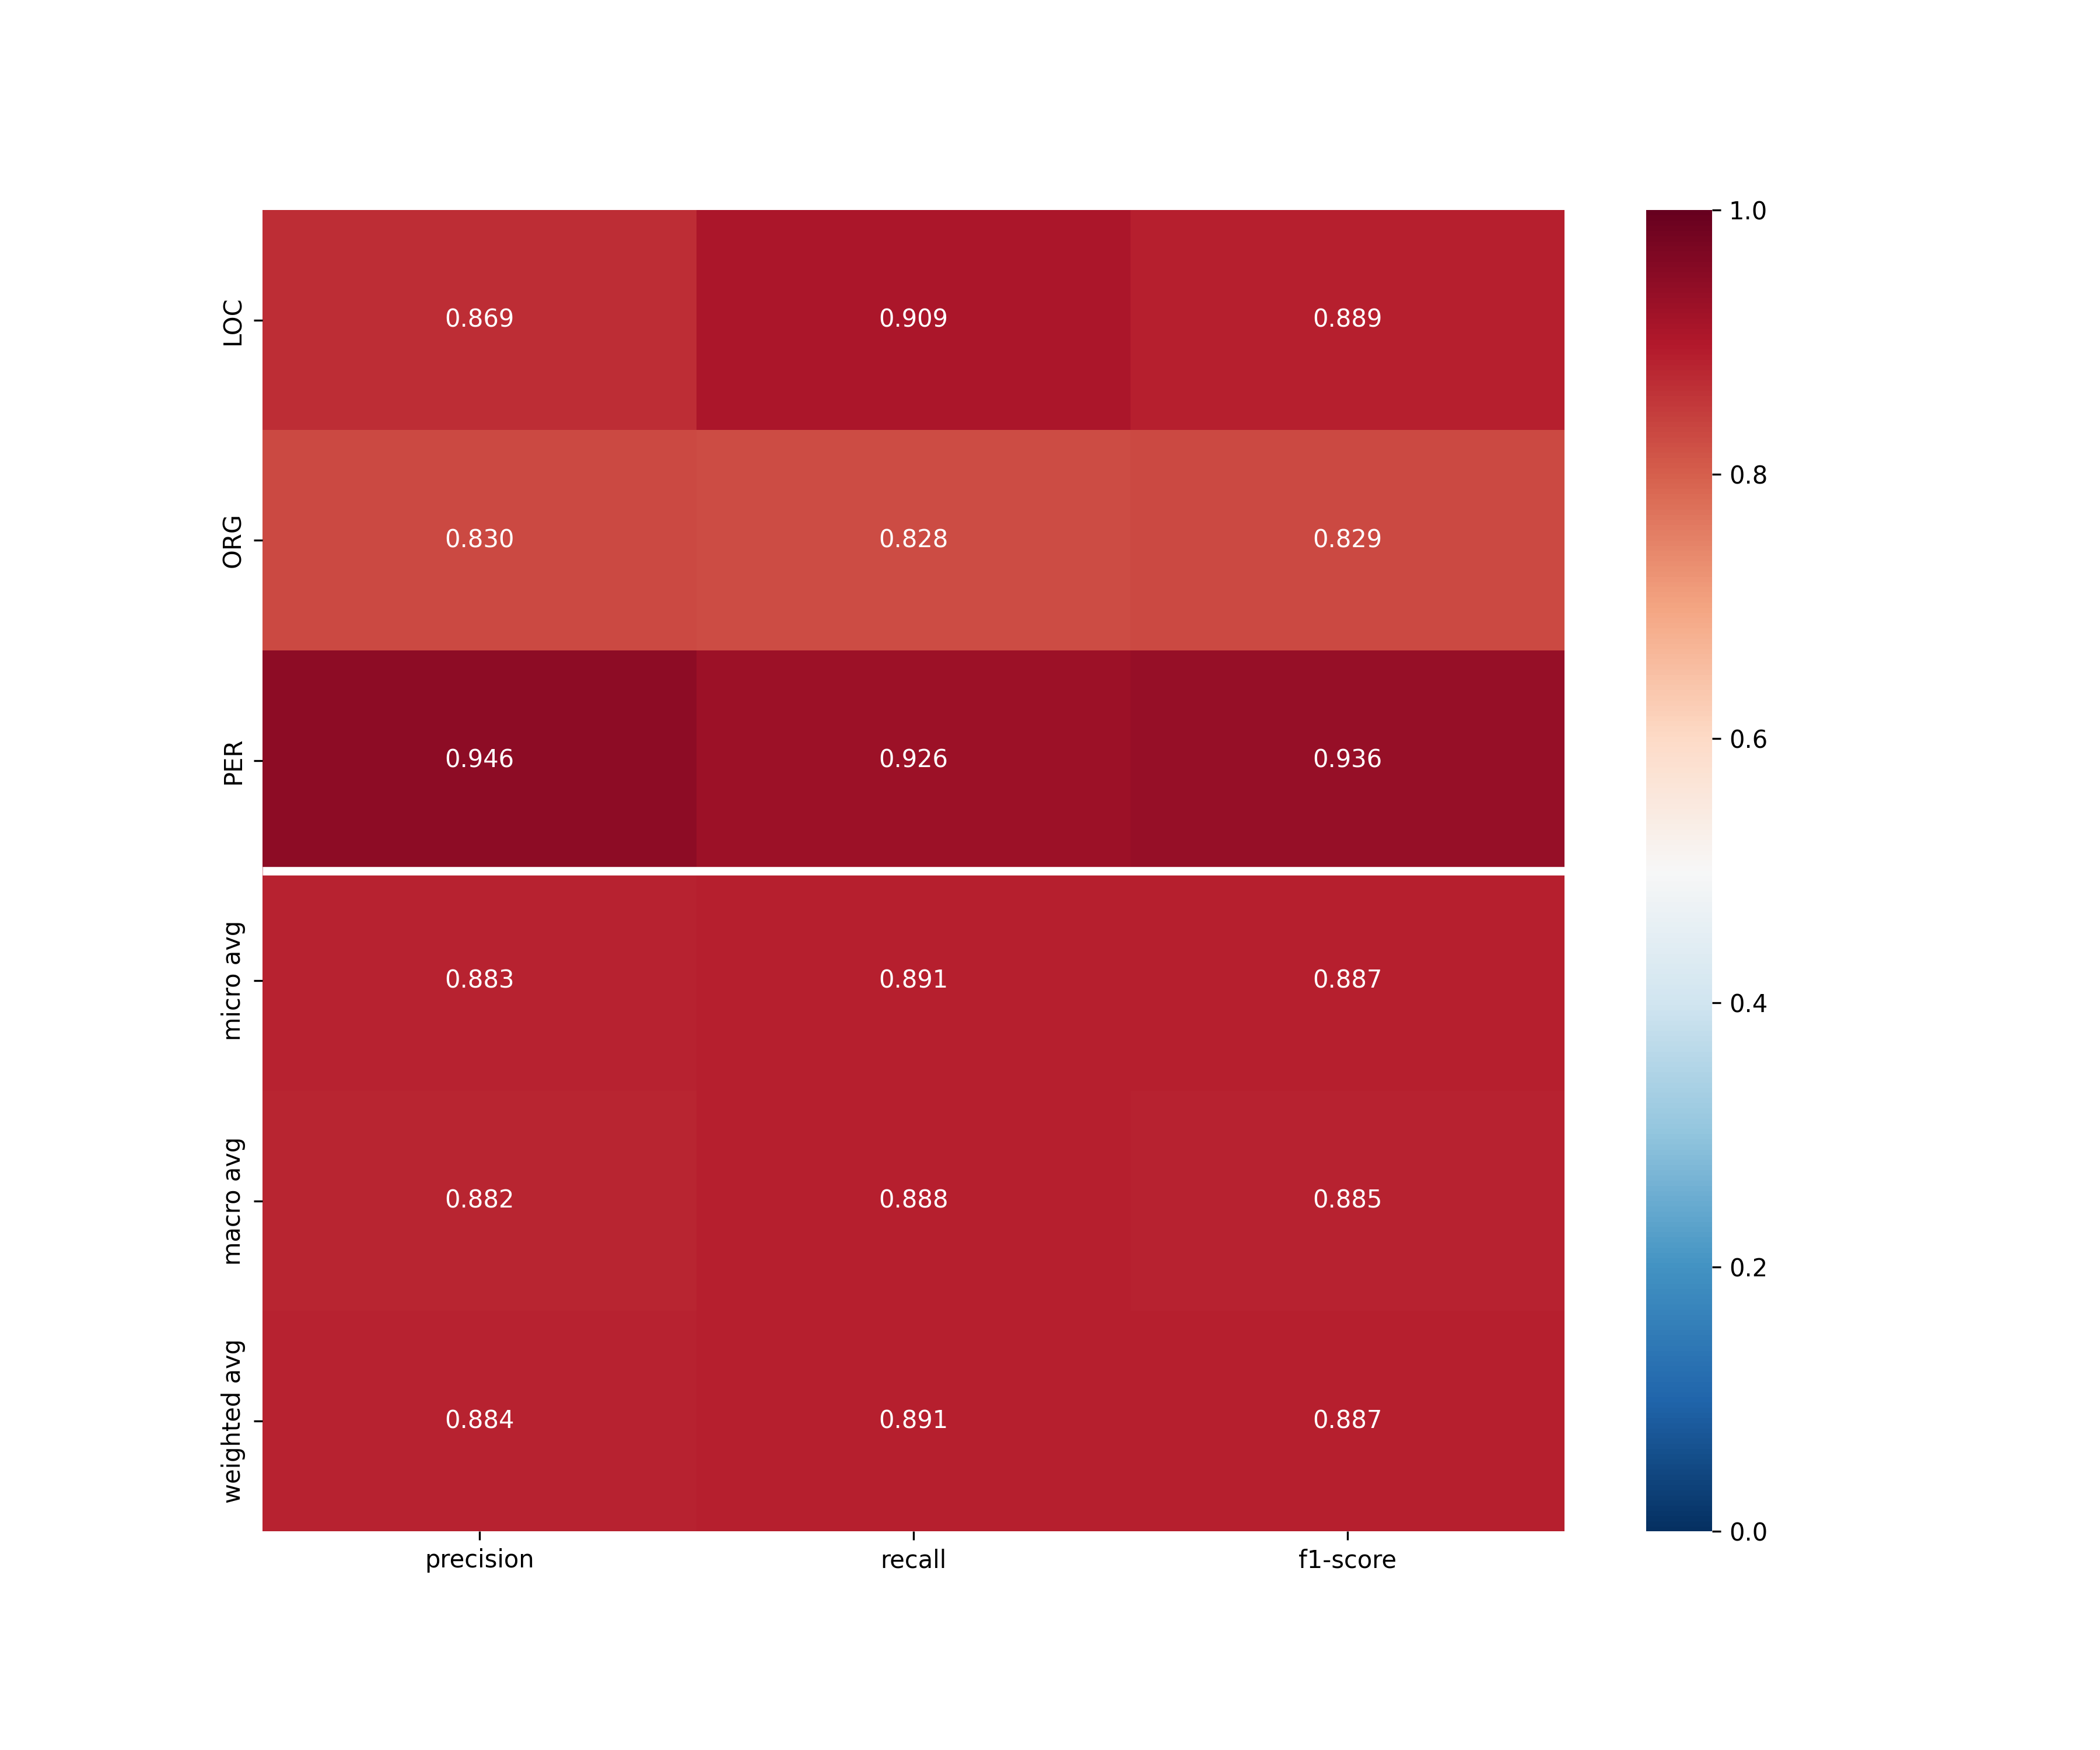
\includegraphics[trim=2cm 0 4cm 0, width=1.0\linewidth]{images/results/author_parser/ner_bert_de_cls_report.png}
    \caption{The resulting precision, recall, and F1-scores of our Author Parser Model used in BiBEx.}
    \label{fig:results_author_cls}
\end{figure}

\FloatBarrier

\section{Extrinsic Evaluation}\label{sec:results_extrinsic}
In this section, we will explain the methods and strategies we employed to evaluate the performance of our overall system. We will discuss the challenges we encountered and the solutions we devised. Our general aim is to assess how effectively our various models and techniques work together.\\
Evaluating the entire system poses a challenge as it requires both visual information, such as images or PDFs, and structured metadata to compare our predictions against. Additionally, to conduct an evaluation of our system, we need metadata containing the authors of an article, as well as segmented and parsed reference entities.\\
However, datasets that fulfill all of these requirements are rare. To address this, we decided to evaluate our system using two distinct datasets. One dataset was used to assess the quality of author extraction, while the other was utilized to evaluate the reference extraction process.

\subsection{Author Extraction}
For the document author evaluation, we curated a corpus by gathering literature from the Social Science Open Access Repository~\cite{noauthor_ssoar_nodate}. The SSOAR provides full-text literature as PDF files, specifically scholarly publications from the domain of social sciences, as well as corresponding metadata.\\
To assemble our corpus, we specifically queried for open access documents related to the field of Geography, ensuring that the file sizes were below 10 MByte to accommodate bandwidth and computational constraints. We processed articles with no more than 30 pages and disregarded those documents, which caused errors during the extraction. This yielded a diverse collection of 2,032 historical and modern-day documents from 2,501 authors, consisting of scientific articles written in various languages, with German and English being the predominant ones. These documents served as the foundation for evaluating the performance of our document author extraction.\\
In our evaluation, we compared our models against the GROBID BiLSTM-CRF and CRF backend as reference models. During the analysis of our corpus, we observed instances where the authors extracted from metadata files did not perfectly align with the corresponding text in the OCR layers. This discrepancy was most likely caused by errors during the OCR process of these articles, like mix-ups between lowercase \enquote{i} and lowercase \enquote{l}.\\
To address this issue and improve the matching criteria, we adopted a two-fold approach. Firstly, we utilized an exact matching criterion where each character of the predicted author and the true author had to coincide for a strict comparison.\\
Secondly, we incorporated the Levenshtein distance~\cite{levenshtein1966binary}, which allowed for a more relaxed matching criteria, enabling us to handle cases with slight differences between the extracted and true authors. The results are shown in Table~\ref{tab:results_overall_author}.

\begin{table}[!ht]
\centering
\begin{tabular}{l|ll|ll|ll|}
\cline{2-7}
                                & \multicolumn{2}{c|}{\textbf{BiBEx}}                                                & \multicolumn{2}{c|}{\textbf{GROBID$^{DL}$}}                                    & \multicolumn{2}{c|}{\textbf{GROBID$^{CRF}$}}                                           \\ \cline{2-7} 
\textbf{}                       & \multicolumn{1}{l|}{exact}                   & loose                   & \multicolumn{1}{l|}{exact}                   & loose                   & \multicolumn{1}{l|}{exact}                   & loose                   \\ \hline
\multicolumn{1}{|l|}{precision} & \multicolumn{1}{l|}{\cellcolor[HTML]{DAE8FC}0.716} & \cellcolor[HTML]{EFEFEF}0.747 & \multicolumn{1}{l|}{\cellcolor[HTML]{DAE8FC}0.377} & \cellcolor[HTML]{EFEFEF}0.389 & \multicolumn{1}{l|}{\cellcolor[HTML]{DAE8FC}0.511} & \cellcolor[HTML]{EFEFEF}0.528 \\ \hline
\multicolumn{1}{|l|}{recall}    & \multicolumn{1}{l|}{\cellcolor[HTML]{DAE8FC}0.703} & \cellcolor[HTML]{EFEFEF}0.734 & \multicolumn{1}{l|}{\cellcolor[HTML]{DAE8FC}0.526} & \cellcolor[HTML]{EFEFEF}0.543 & \multicolumn{1}{l|}{\cellcolor[HTML]{DAE8FC}0.511} & \cellcolor[HTML]{EFEFEF}0.529 \\ \hline
\multicolumn{1}{|l|}{F1-score}  & \multicolumn{1}{l|}{\cellcolor[HTML]{DAE8FC}0.710} & \cellcolor[HTML]{EFEFEF}0.741  & \multicolumn{1}{l|}{\cellcolor[HTML]{DAE8FC}0.439} & \cellcolor[HTML]{EFEFEF}0.453 & \multicolumn{1}{l|}{\cellcolor[HTML]{DAE8FC}0.511} & \cellcolor[HTML]{EFEFEF}0.529 \\ \hline
\end{tabular}
\caption{The resulting precision, recall, and F1-scores of the article author extraction process. We compare BiBEx and GROBID with the BiLSTM-CRF (DL) and CRF backend. The loose matching utilizes a Levenshtein distance of 1, for matching predicted and true authors.}
\label{tab:results_overall_author}
\end{table}

\subsection{Reference Extraction}
To evaluate the quality of our citation metadata extraction process, we utilized the dataset provided by Cioffi et al.~\cite{cioffi2022structured} as a gold standard. This dataset consists of 56 documents, comprising 2,538 reference strings, and encompasses articles from various domains. The authors of this dataset offer open-access articles in the form of PDF files, along with corresponding bibliographic metadata. The dataset is designed as a benchmark for assessing the efficacy of metadata extraction tools of scientific publications.
In their evaluation, the authors propose a 3-fold evaluation methodology, which distinguishes between three metrics:
\newpage

\begin{itemize}
    \item The first evaluation metric focuses on correctly identified references, assessing a tool's capability to distinguish each reference from the surrounding text and other references.
    \item The second evaluation aspect measures the number of correctly tagged metadata entities per reference, irrespective of the correctness of the content itself.
    \item The third evaluation feature measures the number of correctly parsed and tagged contents within each bibliographic reference.
\end{itemize}

After extracting bibliographic references from this dataset, we transformed our outputs from a JSON format to a TEI format to enable a comparison with other systems. Our evaluation involved comparing our results against those obtained from GROBID, CERMINE, ParsCit, and Anystyle, which was found to yield the best overall performance in the evaluation conducted by Cioffi et al. The results are visualized in Table~\ref{tab:results_reference_extraction}.

\begin{table}[!ht]
\begin{tabular}{cl|
>{\columncolor[HTML]{DAE8FC}}l |
>{\columncolor[HTML]{EFEFEF}}l |
>{\columncolor[HTML]{DAE8FC}}l |
>{\columncolor[HTML]{EFEFEF}}l |
>{\columncolor[HTML]{DAE8FC}}l |}
%l|l|l|l|l|}
% >{\columncolor[HTML]{EFEFEF}}l |l|
% >{\columncolor[HTML]{EFEFEF}}l |l|
% >{\columncolor[HTML]{EFEFEF}}l |}
\cline{3-7}
\multicolumn{1}{l}{}                                        & \textbf{} & \textbf{CERMINE} & \textbf{GROBID}        & \textbf{EXCITE} & \textbf{Anystyle}      & \textbf{BiBEx}         \\ \hline
\multicolumn{1}{|c|}{}                                      & precision & 0.75    & 0.54          & 0.59   & 0.81          & \textbf{0.83} \\ \cline{2-7} 
\multicolumn{1}{|c|}{}                                      & recall    & 0.67    & 0.55          & 0.53   & 0.74          & \textbf{0.86} \\ \cline{2-7} 
\multicolumn{1}{|c|}{\multirow{-3}{*}{\textbf{references}}} & F1-score  & 0.71    & 0.54          & 0.56   & 0.77          & \textbf{0.84} \\ \hline\hline
\multicolumn{1}{|c|}{}                                      & precision & 0.94    & 0.86          & 0.93   & 0.93          & \textbf{0.95} \\ \cline{2-7} 
\multicolumn{1}{|c|}{}                                      & recall    & 0.94    & \textbf{0.97} & 0.93   & \textbf{0.97} & \textbf{0.97} \\ \cline{2-7} 
\multicolumn{1}{|c|}{\multirow{-3}{*}{\textbf{metadata}}}   & F1-score  & 0.94    & 0.91          & 0.93   & 0.95          & \textbf{0.96} \\ \hline\hline
\multicolumn{1}{|c|}{}                                      & precision & 0.86    & 0.81          & 0.8    & 0.87          & \textbf{0.88} \\ \cline{2-7} 
\multicolumn{1}{|c|}{}                                      & recall    & 0.87    & \textbf{0.91} & 0.8    & \textbf{0.91} & 0.9           \\ \cline{2-7} 
\multicolumn{1}{|c|}{\multirow{-3}{*}{\textbf{content}}}    & F1-score  & 0.86    & 0.86          & 0.8    & \textbf{0.89} & \textbf{0.89} \\ \hline\hline
\end{tabular}
\caption{The resulting precision, recall, and F1 scores of the BiBEx reference extraction process compared to various other extraction tools.}
\label{tab:results_reference_extraction}
\end{table}